\documentclass{standalone}
\usepackage{tikz}
\usetikzlibrary{patterns, positioning}


\begin{document}
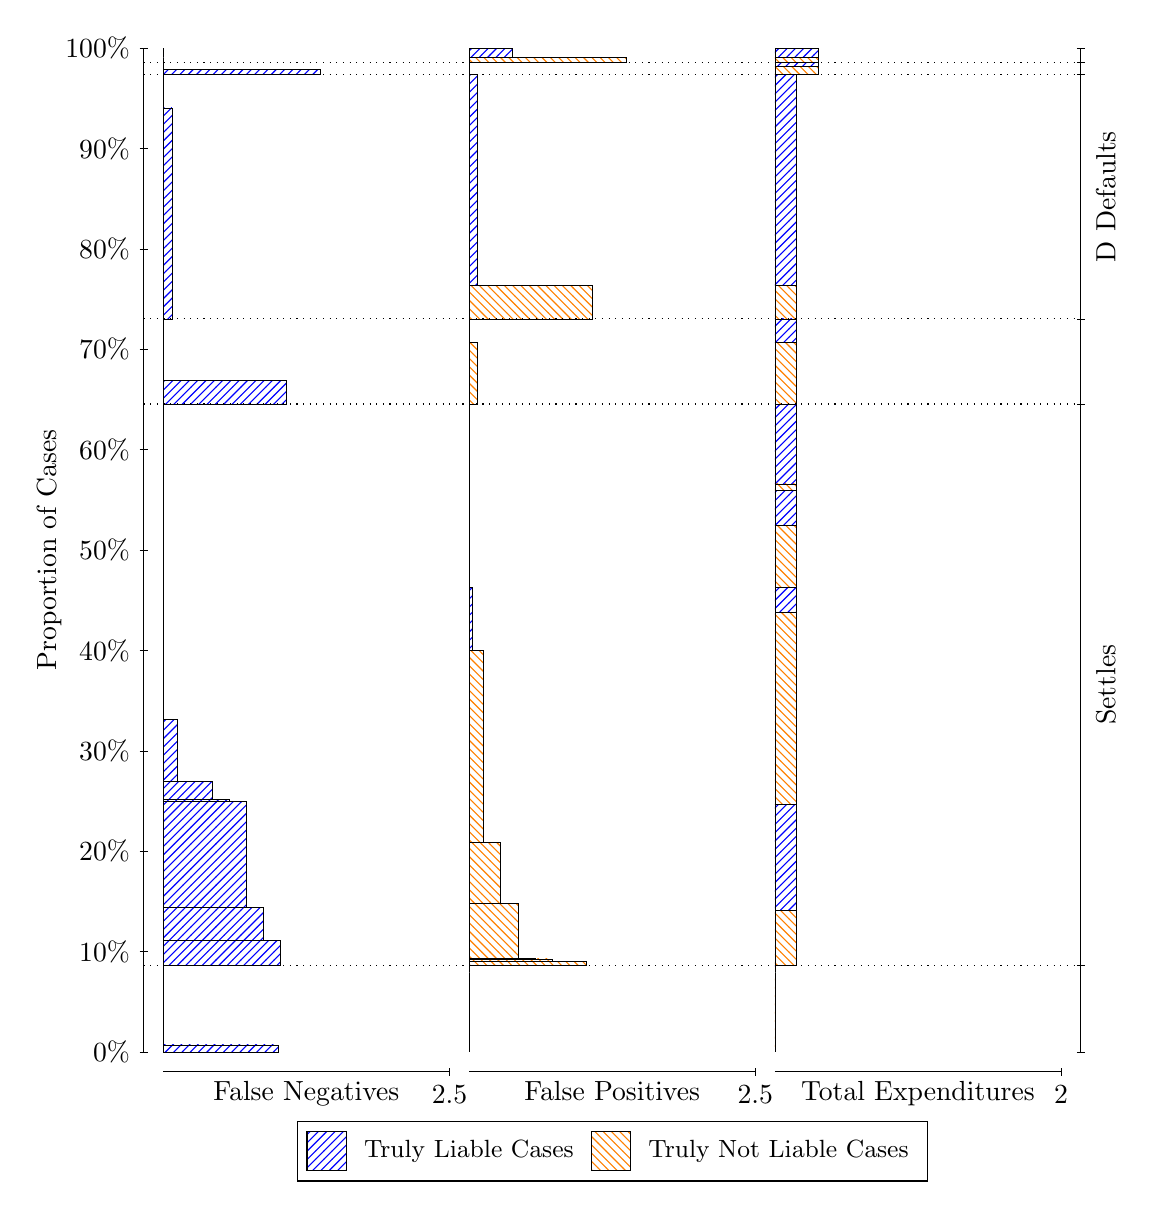
\begin{tikzpicture}
\draw[black, very thin] (1.5,1.75) -- (1.5,14.5);
\node[rotate=90, text=black, anchor=center] at (0.3, 8.125) {Proportion of Cases};
\draw[black, very thin] (1.45,1.75) -- (1.55,1.75);
\node[text=black, anchor=east] at (1.45, 1.75) {0\%};
\draw[black, very thin] (1.45,3.025) -- (1.55,3.025);
\node[text=black, anchor=east] at (1.45, 3.025) {10\%};
\draw[black, very thin] (1.45,4.3) -- (1.55,4.3);
\node[text=black, anchor=east] at (1.45, 4.3) {20\%};
\draw[black, very thin] (1.45,5.575) -- (1.55,5.575);
\node[text=black, anchor=east] at (1.45, 5.575) {30\%};
\draw[black, very thin] (1.45,6.85) -- (1.55,6.85);
\node[text=black, anchor=east] at (1.45, 6.85) {40\%};
\draw[black, very thin] (1.45,8.125) -- (1.55,8.125);
\node[text=black, anchor=east] at (1.45, 8.125) {50\%};
\draw[black, very thin] (1.45,9.4) -- (1.55,9.4);
\node[text=black, anchor=east] at (1.45, 9.4) {60\%};
\draw[black, very thin] (1.45,10.675) -- (1.55,10.675);
\node[text=black, anchor=east] at (1.45, 10.675) {70\%};
\draw[black, very thin] (1.45,11.95) -- (1.55,11.95);
\node[text=black, anchor=east] at (1.45, 11.95) {80\%};
\draw[black, very thin] (1.45,13.225) -- (1.55,13.225);
\node[text=black, anchor=east] at (1.45, 13.225) {90\%};
\draw[black, very thin] (1.45,14.5) -- (1.55,14.5);
\node[text=black, anchor=east] at (1.45, 14.5) {100\%};

\draw[black, very thin] (13.4,1.75) -- (13.4,14.5);
\draw[black, very thin] (13.35,1.75) -- (13.45,1.75);
\node[anchor=west] at (13.35, 1.75) {};
\draw[black, very thin] (13.35,2.8498) -- (13.45,2.8498);
\node[anchor=west] at (13.35, 2.8498) {};
\draw[black, very thin] (13.35,9.9786) -- (13.45,9.9786);
\node[anchor=west] at (13.35, 9.9786) {};
\draw[black, very thin] (13.35,11.061) -- (13.45,11.061);
\node[anchor=west] at (13.35, 11.061) {};
\draw[black, very thin] (13.35,14.165) -- (13.45,14.165);
\node[anchor=west] at (13.35, 14.165) {};
\draw[black, very thin] (13.35,14.32) -- (13.45,14.32);
\node[anchor=west] at (13.35, 14.32) {};
\draw[black, very thin] (13.35,14.5) -- (13.45,14.5);
\node[anchor=west] at (13.35, 14.5) {};

\draw[black, very thin, pattern color=blue, pattern=north east lines] (1.75,1.75) rectangle (3.2033,1.839);
\draw[black, very thin, pattern color=orange, pattern=north west lines] (1.75,1.839) rectangle (1.75,2.8498);
\draw[black, very thin, pattern color=blue, pattern=north east lines] (1.75,2.8498) rectangle (3.2397,3.1666);
\draw[black, very thin, pattern color=blue, pattern=north east lines] (1.75,3.1666) rectangle (3.0217,3.589);
\draw[black, very thin, pattern color=blue, pattern=north east lines] (1.75,3.589) rectangle (2.8037,4.9349);
\draw[black, very thin, pattern color=blue, pattern=north east lines] (1.75,4.9349) rectangle (2.5857,4.9621);
\draw[black, very thin, pattern color=blue, pattern=north east lines] (1.75,4.9621) rectangle (2.3677,5.182);
\draw[black, very thin, pattern color=blue, pattern=north east lines] (1.75,5.182) rectangle (1.9317,5.9747);
\draw[black, very thin, pattern color=orange, pattern=north west lines] (1.75,5.9747) rectangle (1.75,9.9786);
\draw[black, very thin, pattern color=blue, pattern=north east lines] (1.75,9.9786) rectangle (3.3123,10.279);
\draw[black, very thin, pattern color=orange, pattern=north west lines] (1.75,10.279) rectangle (1.75,11.061);
\draw[black, very thin, pattern color=blue, pattern=north east lines] (1.75,11.061) rectangle (1.859,13.741);
\draw[black, very thin, pattern color=orange, pattern=north west lines] (1.75,13.741) rectangle (1.75,14.165);
\draw[black, very thin, pattern color=blue, pattern=north east lines] (1.75,14.165) rectangle (3.7483,14.224);
\draw[black, very thin, pattern color=orange, pattern=north west lines] (1.75,14.224) rectangle (1.75,14.32);
\draw[black, very thin, pattern color=orange, pattern=north west lines] (1.75,14.32) rectangle (1.75,14.379);
\draw[black, very thin, pattern color=blue, pattern=north east lines] (1.75,14.379) rectangle (1.75,14.5);
\draw[black, very thin, pattern color=orange, pattern=north west lines] (5.6333,1.75) rectangle (5.6333,2.7608);
\draw[black, very thin, pattern color=blue, pattern=north east lines] (5.6333,2.7608) rectangle (5.6333,2.8498);
\draw[black, very thin, pattern color=orange, pattern=north west lines] (5.6333,2.8498) rectangle (7.123,2.9012);
\draw[black, very thin, pattern color=orange, pattern=north west lines] (5.6333,2.9012) rectangle (6.687,2.9319);
\draw[black, very thin, pattern color=orange, pattern=north west lines] (5.6333,2.9319) rectangle (6.469,2.9421);
\draw[black, very thin, pattern color=orange, pattern=north west lines] (5.6333,2.9421) rectangle (6.251,3.6395);
\draw[black, very thin, pattern color=orange, pattern=north west lines] (5.6333,3.6395) rectangle (6.033,4.4145);
\draw[black, very thin, pattern color=orange, pattern=north west lines] (5.6333,4.4145) rectangle (5.815,6.8537);
\draw[black, very thin, pattern color=blue, pattern=north east lines] (5.6333,6.8537) rectangle (5.6697,7.6464);
\draw[black, very thin, pattern color=blue, pattern=north east lines] (5.6333,7.6464) rectangle (5.6333,9.9786);
\draw[black, very thin, pattern color=orange, pattern=north west lines] (5.6333,9.9786) rectangle (5.7423,10.76);
\draw[black, very thin, pattern color=blue, pattern=north east lines] (5.6333,10.76) rectangle (5.6333,11.061);
\draw[black, very thin, pattern color=orange, pattern=north west lines] (5.6333,11.061) rectangle (7.1957,11.485);
\draw[black, very thin, pattern color=blue, pattern=north east lines] (5.6333,11.485) rectangle (5.7423,14.165);
\draw[black, very thin, pattern color=orange, pattern=north west lines] (5.6333,14.165) rectangle (5.6333,14.262);
\draw[black, very thin, pattern color=blue, pattern=north east lines] (5.6333,14.262) rectangle (5.6333,14.32);
\draw[black, very thin, pattern color=orange, pattern=north west lines] (5.6333,14.32) rectangle (7.6317,14.379);
\draw[black, very thin, pattern color=blue, pattern=north east lines] (5.6333,14.379) rectangle (6.1783,14.5);
\draw[black, very thin, pattern color=orange, pattern=north west lines] (9.5167,1.75) rectangle (9.5167,2.7608);
\draw[black, very thin, pattern color=blue, pattern=north east lines] (9.5167,2.7608) rectangle (9.5167,2.8498);
\draw[black, very thin, pattern color=orange, pattern=north west lines] (9.5167,2.8498) rectangle (9.7892,3.5472);
\draw[black, very thin, pattern color=blue, pattern=north east lines] (9.5167,3.5472) rectangle (9.7892,4.8932);
\draw[black, very thin, pattern color=orange, pattern=north west lines] (9.5167,4.8932) rectangle (9.7892,7.3324);
\draw[black, very thin, pattern color=blue, pattern=north east lines] (9.5167,7.3324) rectangle (9.7892,7.6491);
\draw[black, very thin, pattern color=orange, pattern=north west lines] (9.5167,7.6491) rectangle (9.7892,8.4343);
\draw[black, very thin, pattern color=blue, pattern=north east lines] (9.5167,8.4343) rectangle (9.7892,8.8839);
\draw[black, very thin, pattern color=orange, pattern=north west lines] (9.5167,8.8839) rectangle (9.7892,8.966);
\draw[black, very thin, pattern color=blue, pattern=north east lines] (9.5167,8.966) rectangle (9.7892,9.9786);
\draw[black, very thin, pattern color=orange, pattern=north west lines] (9.5167,9.9786) rectangle (9.7892,10.76);
\draw[black, very thin, pattern color=blue, pattern=north east lines] (9.5167,10.76) rectangle (9.7892,11.061);
\draw[black, very thin, pattern color=orange, pattern=north west lines] (9.5167,11.061) rectangle (9.7892,11.485);
\draw[black, very thin, pattern color=blue, pattern=north east lines] (9.5167,11.485) rectangle (9.7892,14.165);
\draw[black, very thin, pattern color=orange, pattern=north west lines] (9.5167,14.165) rectangle (10.062,14.262);
\draw[black, very thin, pattern color=blue, pattern=north east lines] (9.5167,14.262) rectangle (10.062,14.32);
\draw[black, very thin, pattern color=orange, pattern=north west lines] (9.5167,14.32) rectangle (10.062,14.379);
\draw[black, very thin, pattern color=blue, pattern=north east lines] (9.5167,14.379) rectangle (10.062,14.5);
\draw[black, dotted] (1.5,2.8498) -- (13.4,2.8498);
\draw[black, dotted] (1.5,9.9786) -- (13.4,9.9786);
\draw[black, dotted] (1.5,11.061) -- (13.4,11.061);
\draw[black, dotted] (1.5,14.165) -- (13.4,14.165);
\draw[black, dotted] (1.5,14.32) -- (13.4,14.32);
\draw[black, very thin] (1.75,1.5) -- (5.3833,1.5);
\node[text=black, anchor=north] at (3.5667, 1.5) {False Negatives};
\draw[black, very thin] (5.3833,1.45) -- (5.3833,1.55);
\node[text=black, anchor=north] at (5.3833, 1.45) {2.5};

\draw[black, very thin] (5.6333,1.5) -- (9.2667,1.5);
\node[text=black, anchor=north] at (7.45, 1.5) {False Positives};
\draw[black, very thin] (9.2667,1.45) -- (9.2667,1.55);
\node[text=black, anchor=north] at (9.2667, 1.45) {2.5};

\draw[black, very thin] (9.5167,1.5) -- (13.15,1.5);
\node[text=black, anchor=north] at (11.333, 1.5) {Total Expenditures};
\draw[black, very thin] (13.15,1.45) -- (13.15,1.55);
\node[text=black, anchor=north] at (13.15, 1.45) {2};


\node[text=black, centered, rotate=90] at (13.72, 6.4142) {Settles};

\node[text=black, centered, rotate=90] at (13.72, 12.613) {D Defaults};



\draw (7.449999999999999,1.5) node[draw=none] (baseCoordinate) {};
\begin{scope}[align=center]
        \matrix[scale=0.5, draw=black, below=0.5cm of baseCoordinate, nodes={draw}, column sep=0.1cm]{
            \node[rectangle, draw, minimum width=0.5cm, minimum height=0.5cm, pattern color=blue, pattern=north east lines] {}; &
            \node[draw=none, font=\small, text=black] (B) {Truly Liable Cases}; &
            \node[rectangle, draw, minimum width=0.5cm, minimum height=0.5cm, pattern color=orange, pattern=north west lines] {}; &
            \node[draw=none, font=\small, text=black] (B) {Truly Not Liable Cases}; \\
            };
\end{scope}

\end{tikzpicture}
\end{document}